%!TEX root = UG_PhD_Defense.tex

\begin{frame}{\large Preliminaries: Finite fields}
\bi
	\item Fields - set of elements over which operations $(+,\cdot,/)$ can be performed 
	\bi
		\item Ex. $\R,\Q,\C$
	\ei
	\pause
	\vspace{0.1in}
	\item Finite fields (Galois fields) - Finite set of elements
	\bi
		\pause
		\item Ex. $\F_q$, where $q=p^n,~p~=~prime,~n \in \Z_{\geq 1}$ 
		\bi
		% \item When $n=1$, $\F_p = \Z_p \pmod{p}$
		\item With $n=1,~and~p=2$, $\F_2 = \B = \{0,1\}$
		\ei
		\pause
		\item On circuits, $p=2$, $n=$ data-operand width
	\ei
	\pause
	\vspace{0.1in}
	\item Hardware cryptography extensively based on $\Fkn$ (we use $\Fkn$)
    % \bi
		% \item $\F_2 \subset \Fkn$, $n>1$
	% \item We are interested in fields of type $\Fkn$
	% \bi
	% 	\item Binary Galois extension fields with characteristic $2$ ($p$)
	% 	\bi
	% 		\item 
	% 		\item Bit-vector of size $n$ represents $2^n$ distinct elements
	% 	\ei
	% 	\item Finite field properties allow elegant application of algebraic geometry techniques
		% \bi
		% 	\item Practical applications to hardware design, debug, verification, and rectification
		% \ei
	% \ei
\ei
\end{frame}

\begin{frame}{\large Motivation: Finite Field Circuits}
\bi
	\item Applications:
	\bi
		\item Cryptography: RSA, Ellyptic Curve Cryptography (ECC) 
		\item Error Correcting Codes, Digital Signal Processing, RFID, etc.
		\pause
		\bi
			\item Crypto-system bugs can leak secret keys [{\it Biham. et al}, Crypto'08]
			\item RFID tag cloning could cause counterfeiting [{\it Batina. et al}, Security'09]
		\ei
		\pause
		\item Large datapath sizes ($n$) in ECC crypto systems 
		\bi
			\item $\Fkn$ with $n=163, 233, 283, 409, 571$ (NIST standard)
		\ei
	\ei
	\pause
	\vspace{0.1in}
	\item Rectification: 
	\bi
		% \item Arithmetic circuits mostly custom designed; potential for errors
		\item Automated debugging
		\item Synthesize sub-functions as opposed to complete redesign
	\ei
\ei
\end{frame}

\begin{frame}{\large Preliminaries: Field Construction}
\bi
	\item $\Fkn = \F_2[x]\pmod{P_n(x)}$ 
	\bi
		\item $P_n(x) \in \F_2[x]$ irreducible polynomial of degree $n$
		\pause
		\item Operations performed $\pmod{P_n(x)}$ 
		\item Coefficients reduced $\pmod{2}$
	\ei
	\pause
	\vspace{0.1in}
	\vspace{0.1in}
	\item Construct $\F_{2^3}$: 
	\bi
		\item Use $P_3(x) = x^3+x+1$ or $P_3(x) = x^3+x^2+1$
		\pause
		\bi
		\item Fields are isomorphic
		\pause
		\item Root of one is not the same as the other
		\ei
	\ei
	% \vspace{0.1in}
    % \bi
		% \item $\F_2 \subset \Fkn$, $n>1$
	% \item We are interested in fields of type $\Fkn$
	% \bi
	% 	\item Binary Galois extension fields with characteristic $2$ ($p$)
	% 	\bi
	% 		\item 
	% 		\item Bit-vector of size $n$ represents $2^n$ distinct elements
	% 	\ei
	% 	\item Finite field properties allow elegant application of algebraic geometry techniques
		% \bi
		% 	\item Practical applications to hardware design, debug, verification, and rectification
		% \ei
	% \ei
\ei
\end{frame}


% \begin{frame}{\large Problem Statement}
% \begin{figure}[hbt]
% \centering
%     \includegraphics[scale = 0.24]{mas_3_ddc_mfr_b.pdf}
%     \caption*{
%     2-bit patch over a 3-bit circuit } 
%     % $f_W: W+ r_3 + \beta \cdot rr_3$}
%     \label{fig:mas_bug_Wb}
% \end{figure}
% \end{frame}

% \begin{frame}{\large Problem Statement and Objective}
% \bi
% 	\item A multivariate specification polynomial $f \in \Fkn$
% 	\bi
% 		\item $n$ is the operand width
% 		% \item Ex. $Z = A \cdot B \pmod{P_n(x)}$ over $\Fkn$
% 	\ei 
% 	\pause
% 	\vspace{0.1in}
% 	\item A faulty circuit implementation $C$ for specification $f$ 
% 	% \bi
% 		% \item Model gates as polynomials over $\Fkn$
% 	% \ei
% 	\pause
% 	\vspace{0.1in}
% 	\item A primitive polynomial $P_n(x)$ used to construct $\Fkn$
% 	\bi
% 		\item $\Fkn = \F_2[x] \pmod{ P_n(x)}$
% 		% \item Let $\ga$ be one of the roots of $P_n(x)$, i.e. $P_n(\ga) = 0$
% 	\ei
% 	\pause
% 	 % , s.t. $P_n(\ga) = 0$
% 	\vspace{0.1in}
% 	\item A set of $m$ targets from $C$
% 	\bi
% 		\item Model it over $\Fkm$ - challenges?
% 	\ei
% 	\pause 
% 	\vspace{0.1in}
% 	\vspace{0.1in}
% 	\item {\bf Check if $C$ is rectifiable at these $m$ targets }
% \ei
% \end{frame}

\begin{frame}{\large Problem Description: Field Containment}
\begin{figure}[hbt]
\centering
\includegraphics[scale=0.26]{mas_3_ddc_mfr_b_bb.pdf}
\caption*{
% ($n$=3) with gate replacement bugs introduced at nets $d_5$ (AND replaced with an OR) and $d_2$ (AND replaced with an XOR), and a wire replacement bug at net $e_0$ (input shorted to $d_0$ instead of $d_1$).
}
\end{figure}
\end{frame}

\begin{frame}{\large Field Containment}
\begin{figure}[hbt]
\centering
    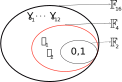
\includegraphics[scale = 0.45]{field_containment.pdf}
    \vspace{0.1in}
    \caption*{\large $\F_2 \subset \F_{4} \subset \F_{16}$}
    \label{fig:field_cont}
\end{figure}
\bi
	\pause
	\item $\F_{2^m} \subset \F_{2^k}$ if $m \mid k$
\ei
\end{frame}

% \begin{frame}{\large Unified framework motivation}
% \bi
% 	% \item A set of $m$ targets from $C$
% 	% \bi
% 	% 	\item Model it over $\Fkm$ - challenges?
% 	% \ei
% 	% \pause 
% 	% \vspace{0.1in}
% 	\item {\bf Check if $C$ is rectifiable at a given set of $m$ targets }
% 	\pause
% 	\vspace{0.1in}
% 	\item Circuit modeled over $\Fkn$ 
% 	\vspace{0.1in}
% 	\bi
% 		\item $P_n(x)$ is given, and let $P_n(\ga) = 0$
% 	\ei
% 	\vspace{0.1in}
% 	\item Rectification patch modeled over $\Fkm$
% 	\vspace{0.1in}
% 	\bi
% 		\item Pick a $P_m(x)$, and let $P_m(\be) = 0$
% 	\ei
% 	\pause 
% 	\vspace{0.1in}
%     \item Single-fix: $m=1,~\forall n \in \Z_{>1}$, $\F_2 \subset \F_{2^n}$, 
% 	\pause
% 	\vspace{0.1in}
% 	\item Multi-fix: $m > 1$, $\Fkm \not\subset \Fkn$
% 	\pause
% 	\bi
% 		\item Ex. For $m=2~and~n=3$, $\F_{2^2} \not\subset \F_{2^3}$
% 	\ei
% 	% \vspace{0.1in}
% 	% \pause
% 	% \item Composite field $\Fkk$ 
% 	% \bi
% 	% 	\item $\Fkm \subset \Fkk$ and $\Fkn \subset \Fkk$, $k=LCM(m,n)$
% 	% \pause
% 	% \vspace{0.1in}
% 	% \item What are the mathematical challenges?
% 	% \pause
% 	% \item What $P_K(x)$ should be used for constructing $\Fkk$
% 	% \ei
% \ei
% \end{frame}


% \begin{frame}{\large Rectification: Intuition}
% %ATPG V() V() = empty
% %we have an algebraic proof which is there in the proposal
% % \bi
% 	% \item Single-fix rectification exists at net $x_i$, {\it iff} $V_{\Fq}(r_L) \cup V_{\Fq}(r_H) =
%  % 		\Fq^{|X_{PI}|} = V(J_0^{PI}) $
% 	\vspace{0.1in}
% 	% Single-fix patch modeled over $\Fkm = \F_{2} (m=1)$ within a circuit 
% 	% modeled over $\Fkn = \F_{2^2}$
% 	\begin{enumerate}
% 		\item Rectification check at net $r_3$: %$W = \{e_3\}$
% 		\bi
% 			\item $J_1 = \langle F_1\rangle$, where $F_1=\{f_1,\dots, f_{26}=r_3+0,\dots, f_{30}\}$
% 			\item $J_2 = \langle F_2\rangle$, where $F_2 = \{f_1,\dots, f_{26}=r_3+1,\dots, f_{30}\}$
% 		\ei
% 		\vspace{0.1in}
% 		\pause
% 		\item Compute $rem_1$ and $rem_2$:
% 		\bi
% 			\item $rem_1 = f \xrightarrow[]{J_1, J_0}_+{(\ga+1)\cdot a_2b_1b_2+(\ga^2+\ga)\cdot a_2b_2}$
% 			\item $rem_2 = f \xrightarrow[]{J_2,J_0}_+{(\ga+1)\cdot a_2b_1b_2+(\ga+1)\cdot a_2b_1+(\ga^2+\ga)\cdot a_2b_2}$
% 		\ei
% 		\vspace{0.1in}
% 		\pause
% 		% \item Single-fix rectification possible iff $G = GB(r1\cdot r2, F_0)=F_0$
% 		\item SFR possible {\bf iff} $V(rem_1) \cup V(rem_2) = \F_{2^3}^{|X_{PI}|} = V(J_0)$
% 		\bi
% 		\pause
% 			\vspace{0.1in}
% 			\item Compute $G = GB(rem_1\cdot rem_2, J_0)$ and check if $G=J_0$
% 			\vspace{0.1in}
% 			\item In this example, target $r_3$ doesn't admit SFR
% 		\ei
% 	\end{enumerate}
% % \ei
% \end{frame}

% \begin{frame}{\large Preliminaries: Variables, Polynomials and Monomial order}
% \bi
% 	\item Let $R=\ftnwring$
% 	\bi
% 		\item $\{f_1, \dots, f_s\} \in R$
% 	\ei
% 	\vspace{0.1in}
% 	\pause
% 	\item In our context
% 	\bi
% 		\item $x_1,\dots,x_d$: Variables (nets of the circuit)
% 		\item $Z$: bit-vector representation for variables
% 		\item $f_1, \dots, f_s$: Polynomials from the circuit (logic gate relations)
% 	\ei
% 	\vspace{0.1in}
% 	\pause
% 	\item Multivariate polynomials: Impose monomial order ``$>$'' on $R$
% 	\bi
% 		\item We utilize lexicographic term order
% 	\ei
% 	\vspace{0.1in}
% 	\pause
%     \item Vanishing Polynomials: $F_0 =  \langle x_1^2+x_1,\dots,x_d^2+x_d, Z^{2^n}+Z\rangle$
% 	\bi
% 		\item Restrict solutions to $x_i$ in $\F_2$
% 		\item Restrict solutions to $Z$ in $\Fkn$
% 	\ei
% \ei
% \end{frame}

% \begin{frame}{\large Algebraic Geometry: Ideals}
% \bi
% 	\item $J = \langle F \rangle = \langle f_1, \dots, f_s \rangle \subseteq R$
% 	\bi
% 		\item $\{h_1f_1 + \cdots + h_sf_s:~h_i \in R\}$
% 		\item Polynomials $f_1, \dots, f_s$: {\it basis} or {\it generators} of $J$
% 	\ei
% 	\vspace{0.1in}
% 	\item Vanishing Ideal: $J_0 = \langle F_0 \rangle =  \langle x_1^2+x_1,\dots,x_d^2+x_d, Z^{2^n}+Z\rangle$
% 	\bi
% 		\item Restrict solutions to $x_i$ in $\F_2$
% 		\item Restrict solutions to $Z$ in $\Fkn$
% 	\ei
% \ei
% \end{frame}

% \begin{frame}{\large Algebraic Geometry: Ideals and Varieties}
% \bi
% 	% \item Let $J = \langle F \rangle = \langle f_1, \dots, f_s \rangle \subseteq R=\ftnwring$
% 	% \vspace{0.1in}
% 	% \item Vanishing Ideal: $J_0 = \langle F_0 \rangle =  \langle x_1^2+x_1,\dots,x_d^2+x_d, Z^{2^n}+Z\rangle$
% 	\item $J = \langle F \rangle = \langle f_1, \dots, f_s \rangle \subseteq \ftnwring $
% 	\bi
% 		\item $\{h_1f_1 + \cdots + h_sf_s:~h_i \in R\}$
% 	\ei
% 	\vspace{0.1in}
% 	\pause
% 	\item Let $\bm{a} = (a_1,\dots,a_d) \in \Fkn^d$ $s.t.$ $f_1(\bm{a}) = \cdots = f_s(\bm{a})=0$
% \ei
% \begin{align*}
% V(J) = \text{Set of all }\{\bm{a}\} \text{ s.t. }\begin{cases}
% f_1(\bm{a}) = 0, \\
% f_2(\bm{a}) = 0, \\
% \vdots \\
% f_s(\bm{a}) = 0
% \end{cases}
% \end{align*}
% \pause
% \bi
% \item $V(J)$ correspond to function mappings (Truth tables)
% \ei
% \end{frame}

% \begin{frame}{\large \Grobner Basis and Ideal membership}
% \bi
% 	\item An ideal can have many generators. 
% 	\vspace{0.1in}
% 	\bi
% 		\item $J = \langle f_1,\dots,f_s\rangle = \langle p_1,\dots,p_m\rangle = \dots = \langle g_1,\dots,g_t\rangle$
% 		\vspace{0.1in}
% 		\item \Grobner Basis (GB) is one such set with special properties
% 		% \bi
% 		% 	\item Presence or absence of solutions (varieties)
% 		% 	% \item Determine dimension of varieties.
% 		% 	\item Ideal membership of a polynomial
% 		% \ei
% 	\ei
% 	\pause
% 	% \bi
% 	% 	\item Same ideal different sets of generators
% 	% \ei
% 	\vspace{0.1in}
% 	\vspace{0.1in}
% 	\item Let $J =  \langle f_1,\dots,f_s\rangle = \langle g_1,\dots,g_t\rangle$
% 	and $G = \{g_1,\dots,g_t \}$.
% 	\bi
% 	\item $G$ is a \Grobner basis of $J \iff \forall f \in J, f \xrightarrow[]{g_1,\dots,g_t}_+ 0$ 
% 	% \ei
% 	\vspace{0.1in}
% 	\item Ideal membership: Let $f$ be a polynomial in $R$:
% 	\bi
% 		\item if $f \xrightarrow[]{g_1,\dots,g_t}_+ 0$, then $f$ is a member of $J$. 
% 	\ei
% 	\ei
% \ei
% \vspace{0.1in}
% \pause
% \begin{figure}
% \centering
% \includegraphics[scale=0.39]{GB.png}
% \end{figure}
% \end{frame}

% \begin{frame}{\large Preliminaries: Term order}
% \bi
% 	\item Reverse Topological Term Order (RTTO)
% 	\bi
% 		\item Exploit circuit structure to avoid expensive GB computation
% 		\item Standard practice to order variables topologically from POs to PIs
% 	\ei
% \ei
% \end{frame}

% \begin{frame}{\large Extended \Grobner Basis}

% \bi
% \item Helps relate an ideal with any generating set contained in the ideal

% %\begin{center}
% \begin{equation*}\label{eqn:matrix}
% \begin{bmatrix} g_1 \\ g_2 \\ \vdots \\ g_t \end{bmatrix}  =  M \cdot
% \begin{bmatrix} f_1 \\ f_2 \\ \vdots \\ f_s \end{bmatrix}
% \end{equation*}
% \item M is a $t\times s$ matrix of polynomials

% \item if $f \in J$, then
% \bi
% \item $f = u_1g_1 + u_2g_2+ \dots+ u_tg_t$
% \item $f = v_1f_1 +\dots+v_sf_s$
% \ei
% \item Used in computation of rectification function
% \ei
% \end{frame}


%How are two ideals and their varieties related? 
%Analyzing Ideal 𝐽 is not enough Need to analyze ideal 𝐼(𝑉( 𝐽))
%SNS reasons about the ideal of polynomials that vanish on V(J).


% \begin{frame}{\large Strong Nullstellensatz}
% \bi
% \item Given an ideal $J\subset R$ and $V(J) \subseteq \Fq^d$ 
% % the {\it ideal of polynomials that vanish on} $V(J)$ is 
% \bi
% 	\item $I(V(J)) = \{ f \in R : \forall \bm{a} \in V(J), f(\bm{a}) = 0\}$.
% \ei

% \item If $f$ vanishes on $V(J)$, then $f \in I(V(J))$. 

% \item The Strong Nullstellensatz characterizes $I(V(J))$ over $\Fq$
% \bi
% 	\item Over finite fields $\Fq$, $I(V_{\Fq}(J)) = J + J_0$.
% 	\item We will use this to formulate rectification check
% \ei
% \ei
% \end{frame}